\chapter{The Zeta Function of Riemann (Contd)}\label{chap10}

\setcounter{section}{1}
\section{(Contd). Elementary theory of Dirichlet  series}\label{chap10:sec2}\pageoriginale

We wish to prove a formula for the partial sum of a Dirichlet
series. We shall give two proofs, one based on an estimate of the
order of the sum-function \cite{key10}, and another
\cite[Lec. \ref{chap4}]{key14}  which is independent of such an estimate. We
first need the following 

\setcounter{lem}{0}
\begin{lem}\label{chap10:lem1}
If $\sigma >0$, then 
$$
\frac{1}{2\pi i } \int\limits^{\sigma + i \infty}_{\sigma - i \infty}
\frac{e^{us}}{s} ds =
\begin{cases}
1, & \text{ if } u > 0\\
0, & \text{ if } u < 0\\
\frac{1}{2}, & \text{ if } u = 0
\end{cases}
$$
where $\int\limits^{\sigma + i \infty}_{\sigma -i \infty} =
\lim\limits_{T \to \infty} \int\limits^{\sigma + i T}_{\sigma -iT}$.
\end{lem}

\begin{proof}
The case $u=0$ is obvious. We shall therefore study only the cases $u
\gtrless 0$. Now
$$
\int\limits^{\sigma + i T}_{\sigma - i T} \frac{e^{us}ds}{s}
=\frac{e^{us}}{us} \int\limits^{\sigma + i T}_{\sigma - i T} +
\int\limits^{\sigma+iT}_{\sigma - iT} \frac{e^{us}}{us^2} ds 
$$ 
\begin{figure}[H]
\centering
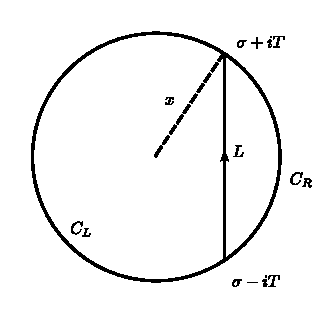
\includegraphics{figures/fig1.eps}
\end{figure}

However
$$
|e^{u(\sigma + i T)}| = e^{u\sigma}
$$
and $|s|>T$; hence, letting $T \to \infty$, we get
$$
\int\limits^{\sigma + i \infty}_{\sigma-i\infty} \frac{e^{us}ds}{s} =
\int\limits^{\sigma + i \infty}_{\sigma - i \infty}
\frac{e^{us}}{us^2} ds \equiv I, \text{ say}.
$$

We shall\pageoriginale evaluate $I$ on the contour suggested by the
diagram. If $u <0$ , we use the contour $L + C_R$; and if $u>0$, we
use $L+C_L$.

If $u<0$, we have, on $C_R$,
$$
\left|\frac{e^{us}}{s^2} \right| \leq \frac{e^{u\sigma}}{r^2}, \text{
  since } \re s > \sigma. 
$$

If $u>0$, we have, on $C_L$,
$$
\left|\frac{e^{us}}{s^2} \right| \leq \frac{e^{u\sigma}}{r^2}, \text{
  since }\re s < \sigma.
$$

Hence
$$
\left|\, \int\limits_{C_R, C_L} \frac{e^{us} ds}{us^2}
\right| \leq 2 \pi r \cdot \frac{e^{u\sigma}}{|u|r^2} \to 0,
\text{ as } r \to \infty.
$$

By Cauchy's theorem, however, we have
$$
\int\limits_L = - \int\limits_{C_R};
$$
hence
$$
(1) \hspace{2.5cm} \frac{1}{2\pi i} \int\limits^{\sigma + i \infty}_{\sigma - i
  \infty} \frac{e^{us}}{us^2} ds = 0, \quad \text{ if } u < 0. \hspace{2.5cm}
$$
If, however, $u>0$, the contour $L + C_L$ encloses a pole of the
second order at the origin, and we get
$$
\int\limits_L = - \int\limits_{C_L} + 1, 
$$
so that
$$
(2) \hspace{2.5cm} \frac{1}{2\pi i} \int\limits^{\sigma + i
  \infty}_{\sigma - i   \infty} \frac{e^{us}}{us^2} ds = 1, \quad
\text{if } u > 0. \hspace{2.5cm}
$$
\end{proof}

\begin{remarks*}
We can\pageoriginale rewrite the Lemma as: if $a>0$,
$$
\frac{1}{2\pi i} \int\limits^{a+i\infty}_{a - i \infty}
\frac{e^{(\lambda - \lambda_n)s}}{s} ds = \begin{cases}
0, & \text{ if } \lambda < \lambda_n\\
1, & \text{ if } \lambda > \lambda_n\\
\frac{1}{2}, & \text{ if } \lambda = \lambda_n
\end{cases}
$$
{\em Formally}, therefore, we should have 
\begin{align*}
\frac{1}{2\pi i} \int\limits^{a+i\infty}_{a-i\infty} f (s)
\frac{e^{\lambda s}}{s} ds & = \frac{1}{2\pi i} \sum\limits^\infty_1
a_n \int\limits^{a+i\infty}_{a-i\infty}
\frac{e^{(\lambda-\lambda_n)s}}{s} ds\\
& = {\mathop{\sum\limits}_{\lambda_n \leq \lambda}} ' a_n
\end{align*}
the dash denoting that if $\lambda =\lambda_n$ the last term should be
halved. We wish now to establish this on a rigorous basis.

We proceed to prove another lemma first.
\end{remarks*}

\begin{lem}\label{chap10:lem2}
Let $\sum a_n e^{-\lambda_ns}$ converge for $s = \beta$ real. Then
$$
\sum\limits^n_1 a_\nu e^{-\lambda_\nu s} = o(|t|),
$$
the estimate holding uniformly both in $\sigma \geq \beta +
\epsilon > \beta$ and in $n$. In particular, for $n = \infty$,
$f(s)=o(|t|)$ uniformly for $\sigma \geq \beta + \epsilon > \beta$ 
\end{lem}

\begin{proof}
Assume that $\beta =0$, without loss of generality. Then 
$$
a_\nu = O(1) \text{ and } A(\lambda_\nu) - A(\lambda_\mu) = O(1)
\text{ for {\bf all} } \nu \text{ and } \mu
$$
If $1< N < n$, then
\begin{align*}
\sum\limits^n_1 a_\nu e^{-\lambda_\nu s} & = \sum^N_1 + \sum^n_{N+1}
a_\nu e^{-\lambda_\nu s}\\
& = \sum^N_1 a_\nu e^{-\lambda_\nu s} + s
\int\limits^{\lambda_n}_{\lambda_N} \{A(x) - A (\lambda_N)\} e^{-xs}
dx\\
&\qquad\qquad \{A(\lambda_n) - A (\lambda_N)\}e^{-\lambda_ns}\\
& = O(N) + O(1) + O\left(|s|
\int\limits^{\lambda_n}_{\lambda_N}e^{-x\sigma}  dx
\right)\\
& = O(N) + O \left(\frac{|s|}{\sigma} e^{-\lambda_N \sigma}  \right)\\
& = O(N) + O \left(|t| e^{-\lambda_N\epsilon} \right)
\end{align*}\pageoriginale 
since $|s|^2 = t^2 + \sigma^2$ and $\sigma \geq \epsilon$.

Hence
$$
\sum\limits^n_1 a_\nu e^{-\lambda_\nu s} = O(N) + O (|t|
e^{-\lambda_N\epsilon}) , \text{ if } 1 < N < n
$$
If $N \geq n$, then, trivially, 
$$
\sum\limits^n_1 a_\nu e^{-\lambda_\nu s} = O (N).
$$
If we choose $N$ as a function of $|t|$, tending to $\infty$ more
slowly than $|t|$, we get
$$
\sum\limits^n_1 a_\nu e^{-\lambda_\nu s} = O (|t|)
$$
in either\pageoriginale case.
\end{proof}

\begin{theorem*}[(Perron's Formula)]
Let $\sigma_0$ be the abscissa of convergence of $\sum a_n
e^{-\lambda_n s}$ whose sum-function is $f(s)$. Then for $\sigma >
\sigma_0$ and $\sigma>0$, we have 
$$
{\sum\limits_{\lambda_\nu \leq \omega}}' a_n = \frac{1}{2\pi i}
\int\limits^{\sigma + i \infty}_{\sigma - i \infty} \frac{f(s)}{s}
e^{\omega s} ds , 
$$
where the dash denotes the fact that if $\omega = \lambda_n$ the last
term is to be halved.
\end{theorem*}


\begin{proof}
Let $\lambda_m \leq \omega < \lambda_{m+1}$, and
$$
g(s) = e^{\omega s} \left\{f(s) - \sum\limits^m_1 a_n e^{-\lambda_n s}
\right\} 
$$
(This has a meaning since $\re s \equiv \sigma > \sigma_0$). Now 
\begin{align*}
& \frac{1}{2\pi i} \int\limits^{\sigma + i \infty}_{\sigma - i \infty}
\frac{g(s)}{s} ds
 = \frac{1}{2\pi i} \int\limits^{\sigma + i \infty}_{\sigma -
i \infty} \frac{f(s) e^{\omega s}}{s} ds - {\mathop{\sum\limits}_{\lambda_n \leq
  \omega}}' a_n
\end{align*}
by the foregoing lemma. We have to show that the last expression is
zero. 

Applying Cauchy's theorem to the rectangle
$$
\sigma-i T_1, \sigma + i T_2, \Omega + i T_2, \Omega -i T_1,
$$
where $T_1 ,T_2 >0$, and $\Omega>\sigma$, we get
$$
\frac{1}{2\pi i} \int\limits^{\sigma + i \infty}_{\sigma - i \infty}
\frac{g(s)}{s} ds = 0,
$$
for\pageoriginale
\begin{align*}
\frac{1}{2\pi i} \int\limits^{\sigma + i T_2}_{\sigma - i T_1} & =
\frac{1}{2\pi i} \left[ \int\limits^{\Omega - i T_1}_{\sigma - i T_1}
  + \int\limits^{\Omega + i T_2}_{\Omega - i T_1} +
  \int\limits^{\sigma + i T_2}_{\Omega + i T_2} \right]\\
& = I_1 + I_2 + I_3, \text{ say}.
\end{align*}

Now, if we fix $T_1$ and $T_2$ and let $\Omega \to \infty$, then we
see that $I_2 \to 0$, for $g(s)$ is the sum-function of
$\sum\limits^\infty_1 b_n^{-\mu_n s}$, where $b_n = a_{m+n}$, $\mu_n =
\lambda_{m+n} - \omega$, with $\mu_1 > 0$, and hence $g(s) = o(1)$ as
$s \to \infty$ in the angle $|am s| \leq \dfrac{\pi}{2} - \delta$.

Thus
$$
\frac{1}{2\pi i} \int\limits^{\sigma + i T_2}_{\sigma - i T_1}
\frac{g(s)}{s} ds = \frac{1}{2\pi i} \left[\int\limits^{\infty - i
    T_1}_{\sigma - i T_1} - \int\limits^{\infty + i T_2}_{\sigma + i
    T_2} \right] 
$$
if the two integrals on the right converge. 

Now if 
$$
h(s) \equiv g(s) e^{(\lambda_{m+1}-\omega)s} = a_{m+1} + a_{m+2}
e^{-(\lambda_{m+2} - \lambda_{m+1})s} + \cdots
$$
then by lemma \ref{chap10:lem2}, we have
$$
|h(s)| < \epsilon T_2
$$
for $s = \sigma + i T_2 $, $\sigma \geq \sigma_0 + \epsilon$,
$T_2 \geq T_0$. Therefore for the second integral on the\pageoriginale
right we have
$$
\left|\int\limits^{\infty + i T_2}_{\sigma + i T_2} \frac{g(s)}{s} ds
\right|  < \frac{\epsilon T_2}{\sqrt{\sigma^2 + T^2_2}}
\int\limits^\infty_\sigma e^{-\mu_1 \xi} d\xi < \epsilon /\mu_1
$$
$\mu_1 > 0$. This proves not only that the integral converges for a
finite $T_2$, but also that as $T_2 \to \infty$, the second integral
tends to zero. Similarly for the first integral on the right.
\end{proof}

\medskip
\noindent{\textbf{N.B.}}
An estimate  for $g(s)$ alone (instead of $h(s)$) will not work!

\begin{remarks*}
More generally we have for $\sigma > \sigma_0$ and $\sigma >
\sigma^\ast$
\begin{gather*}
{\mathop{\sum\limits}_{\lambda_n \leq \omega}}' a_n e^{-\lambda_n s^\ast}  =
\frac{1}{2\pi i} \int\limits^{\sigma + i
  \infty}_{\sigma - i \infty} \frac{f(s)}{s-s^\ast} e^{\omega
  (s-s^\ast)}ds,\\
\text{for } \sum a_n e^{-\lambda_n s^\ast} \cdot e^{\lambda_n(s-s^\ast)} =
\sum a_n  e^{-\lambda_n s} = f(s), 
\end{gather*}
and writing $s'=s-s^\ast$ and $b_n = a_n e^{-\lambda_ns^\ast}$, we
have $f(s) \equiv f(s') = \sum b_n e^{-\lambda_ns'}$.

We shall now give an alternative proof of Person's formula
\textit{without} using the order of $f(s)$ as $s \to \infty$
\cite[Lec. \ref{chap4}]{key14} 
\end{remarks*}

\medskip
\noindent{\textbf{Aliter.}}
If $f(s) = \sum\limits^\infty_1 a_n e^{-\lambda_ns}$ has $\sigma_0
\neq \infty$ as its abscissa of convergence, and if $a>0$,
$a>\sigma_0$, then for $\omega \neq \lambda_n$, we have
$$
\sum\limits_{\lambda_n < \omega} a_n = \frac{1}{2\pi i}
\int\limits^{a+i\infty}_{a-i\infty} f(s) \frac{e^{\omega s}}{s} ds
$$

\begin{proof}
Define\pageoriginale 
\begin{align*}
f_m(s) & = \sum\limits^m_1 a_n e^{-\lambda_ns}\\
\text{and } \qquad \qquad r_m (s) & = \sum\limits^\infty_{m+1} a_n.
e^{-\lambda_ns} = f(s) - f_m(s)
\qquad \qquad 
\end{align*}

Then
$$
(A) \quad \frac{1}{2\pi i} \int\limits^{a+iT}_{a-iT} f(s) \frac{e^{\omega
    s}}{s} ds = \frac{1}{2\pi i} \int\limits^{a+iT}_{a-iT} f_m (s)
\frac{e^{\omega s}}{s} ds + \frac{1}{2\pi i} \int\limits^{a+iT}_{a-iT}
r_m (s) \frac{e^{\omega s}}{s} ds
$$
Here the integral on the left exists since $f(s)$ is regular on
$\sigma = a > \sigma_0$. By Lemma \ref{chap10:lem1}, as applied to the first integral
on the right hand side, we get
$$
(B) \quad \lim\limits_{T \to \infty} \frac{1}{2 \pi i}
\int\limits^{a+iT}_{a-iT} f(s) \frac{e^{\omega s}}{s} ds -
\sum\limits_{\lambda_n < \omega} a_n = \lim\limits_{T\to\infty}
\frac{1}{2\pi i} \int\limits^{a+iT}_{a-iT} r_m (s) \frac{e^{\omega
    s}}{s} ds
$$
the limits existing.

Since $\lambda_n \to \infty$, we can choose $m_0$ such that for all $m
\geq m_0$ we have $\lambda_m > \omega$. For all such $m$ the last
relation holds.

Now write $b_n = a_n e^{-\lambda_n \sigma'}, \phi (x) =
e^{-x(s-\sigma')} $, so that $\sum a_n e^{-\lambda_ns} = \sum b_n \phi
(\lambda)$. Write $B(x) = \sum\limits_{n \leq x} b_n$.

Then applying the Lemma of the \ref{chap9}th lecture, we get
\begin{align*}
\sum^N_{m+1} a_n e^{-\lambda_n s} & = \sum^N_1 - \sum^m_1 \\
& = (s-\sigma') \int\limits^{\lambda_N}_{\lambda_m} B(x)
e^{-x(s-\sigma')} \, dx \\
& \qquad  \qquad + B (\lambda_N) e^{-\lambda_N(s-\sigma')}
-B(m)e^{-\lambda_m(s-\sigma')} \\
& = \{B(\lambda_N) - B (\lambda_m)\} e^{-\lambda_N(s-\sigma')}\\
& \qquad \qquad +(s-\sigma')
  \int\limits^{\lambda_N}_{\lambda_m} \{B(x)  -
B(\lambda_m)\} e^{-x(s-\sigma')} \, dx. 
\end{align*}\pageoriginale 

Now choose $\sigma'>0$ and $a > \sigma' > \sigma_0$. [If $\sigma_0
  \geq 0$ the second condition implies the first; if $\sigma_0 < 0$,
  then since $a>0$, choose $0< \sigma'<a$].

Then $B(x)$ tends to a limit as $x \to \infty$, so that 
$B(x) = o(1)$ \textit{for all $x$}; while $|e^{-x(s-\sigma')}| =
e^{-x(\sigma-\sigma')} \to 0$ as $x \to \infty$ for $\sigma >
\sigma'$. Hence, letting $N \to \infty$, we get
$$
r_m (s) = (s-\sigma') \int\limits^\infty_{\lambda_m} \{B(x) -
B(\lambda_m)\} e^{-x(s-\sigma')} dx,
$$
or
$$
|r_m(s)| \leq c \frac{|s-\sigma'|}{\sigma-\sigma'}
e^{-\lambda_m(\sigma-\sigma')} 
$$

Now consider
$$
\frac{1}{2\pi i} \int\limits_{L+C_R} r_m(s) \frac{e^{\omega s}}{s} ds
$$
where $L+C_R$ is the contour indicated in the diagram.
\begin{figure}[H]
\centering
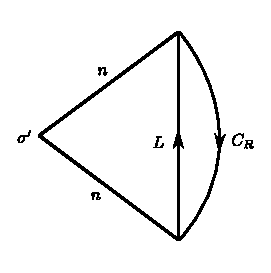
\includegraphics{figures/fig2.eps}
\end{figure}

$r_m(s)$ is\pageoriginale regular in this contour, and the integral is
therefore zero. Hence
$$
\int\limits_L = -\int\limits_{C_R}
$$
On $C_R$, however, $s = \sigma'+ re^{i\theta}$ and $\sigma \geq a$, so
that 
\begin{align*}
|r_m(s)| & \leq c \cdot \frac{r}{a-\sigma'} \cdot e^{-\lambda_m r
  \cos\theta} \\
|e^{\omega s}| & = e^{\omega(\sigma'+r\cos \theta)}, |s| \geq r.\\
\end{align*}

Hence
\begin{align*}
\left|\frac{1}{2\pi i} \int\limits_{C_R} r_m(s) \frac{e^{\omega s}}{s}
ds\right| & \leq \frac{cr}{2\pi (a-\sigma')} e^{\omega \sigma'}
\int\limits^{\pi/2}_{-\pi/2}  e^{(\omega-\lambda_m) r\cos \theta} d
\theta\\
& = \frac{cr}{\pi (a-\sigma')} e^{\omega \sigma'}
\int\limits^{\pi/2}_0 e^{(\omega -\lambda_m) r \sin \theta} d \theta
\end{align*}

However, $\sin \theta \geq \dfrac{2\theta}{\pi}$ for $0 \leq \theta
\leq \pi/2$; hence
\begin{align*}
\left|\frac{1}{2\pi i} \int\limits^{a+iT}_{a-iT} r_m(s)
\frac{e^{\omega s}}{s} ds \right| & \leq \frac{cr e^{\omega
    \sigma'}}{\pi(a-\sigma')} \int\limits^{\pi/2}_0
e^{\frac{2}{\pi}(\omega - \lambda_m)r\theta} d\theta\\
& \leq \frac{cr e^{\omega \sigma'}}{2(a-\sigma')(\lambda_m -\omega)r} \; ,
\end{align*}
for all $T$. Hence
$$
(C) \hspace{2cm} \overline{\lim\limits_{T\to\infty}}
\left|~\int\limits^{a+iT}_{a-iT} r_m(s) \frac{e^{\omega s}}{s}
ds\right|  \leq \frac{c_1}{(\lambda_m - \omega)}
\hspace{2cm}
$$\pageoriginale 
for \textit{all} $m \geq m_0$.

Now reverting to relation (A), we get
\begin{align*}
(D) \quad &\overline{\lim\limits_{T \to \infty}} \left|\frac{1}{2\pi i}
\int\limits^{a+iT}_{a-iT} f(s) \frac{e^{\omega s}}{s}  ds -
\frac{1}{2\pi i} \int\limits^{a+iT}_{a-iT} f_m (s) \frac{e^{\omega
    s}}{s} ds\right|\\  
&\hspace{4cm} = \overline{\lim\limits_{T\to \infty}} \left|
\frac{1}{2\pi i} \int\limits^{a+iT}_{a-iT} r_m(s) \frac{e^{\omega
    s}}{s} ds\right| 
\end{align*}
for every $m$. However,
$$ 
\lim\limits_{T\to\infty} \frac{1}{2\pi i}
\int\limits^{a+iT}_{a-iT} f_m(s) \frac{e^{\omega s}}{s} ds
=\sum\limits_{\lambda_n < \omega} a_n
$$
independently of $m$. Hence\footnote{We use the fact that if 
$$
\overline{\lim\limits_{T \to \infty}} |f(T) - g(T)| = \alpha
$$
and $\lim\limits_{T\to\infty} g(T) = \beta$, then
$$
\overline{\lim\limits_{T\to\infty}} |f(T)-\beta| \leq \alpha 
$$}
\begin{align*}
 \overline{\lim\limits_{T \to \infty} } \left| \frac{1}{2\pi i} \int\limits^{a+iT}_{a-iT} f(s)  \frac{e^{\omega s}}{s} ds  - \sum\limits_{\lambda_n < \omega} a_n \right| &\leq \text{ left hand side in (D)}\\
& \leq \frac{c_1}{\lambda_m - \omega} \text{ for } m > m_0. 
\end{align*}

Letting\pageoriginale $m \to \infty$ we get the result. 
\end{proof}

\begin{remarks*}
\begin{itemize}
\item[{\rm (i)}] If $\omega = \lambda_n$ the last term in the sum
  $\sum\limits_{\lambda_n < \omega}a_n$ has to be multiplied by
  $\dfrac{1}{2}$.

\item[(ii)] If $a<0$, (and $a>\sigma_0$) then in the
  contour-integration the residue at the origin has to be taken, and
  this will contribute a term - $f(0)$. In the proof, the relation
  between $|s|$ and $r$ has to be modified. 
\end{itemize}
\end{remarks*}
